\documentclass{beamer}
\usepackage[utf8]{inputenc}
\usepackage{graphicx}
\usetheme{Szeged}
\usecolortheme{wolverine}
\title{Probabilistic Dust Storm Prediction}
\subtitle{Context-Senstive Impact Discovery}
\author{Sean Flaherty}
\date{2017}

\begin{document}
\begin{frame}
	\titlepage
	Mentors: Dr. Huiping Cao, Dr. Colby Brungard, Dr. David DuBois\\
	Acknowledgements: Josue Gutierrez, Merrill Bean, Max Bleiweiss

\end{frame}
\begin{frame}
	\frametitle{Motivation}
	\begin{itemize}
		\item
			Dust storms are a hazard to public health and economic development where they occur.
		\item
			Predictive models paired with communication systems allow for an early warning system to prepare for and reduce potential damage [1].
	\end{itemize}

\end{frame}
\begin{frame}
	\frametitle{Overview}
	\begin{itemize}
		\item
			Goal: Use data mining/machine learning to create a predictive model for dust events on a local scale.
		\item
			Previous research: Univariate predictor (500mB geopotential height) using image processing (ZNCC). Only good at predicting large events [2]. 
		\item
			Justification: Want an accurate predictor for meso- and micro-scale dust events.
	\end{itemize}

\end{frame}
\begin{frame}
	\frametitle{Gathering Data}
	\begin{itemize}
		\item<-1->
			RAP/RUC forecast model -- NOMADS (NOAA Operational Model Archive and Distribution System).
		\item<-2-> Forecasts available from NOAA online repository (HTTPS/FTP).
		\item<-3-> Data downloaded using GNU wget utility [3].
	\end{itemize}
\end{frame}
\begin{frame}
	\frametitle{Data Format}
	\begin{itemize}
		\item
			GRIB -- GRIdded Binary (WMO standard for weather data).
		\item
			RAP/RUC models update forecasts hourly with 13 and 25.2 km resolutions.
		\ite
			Each file contains forecast models for a single time.
		\item
			Each file has a number of weather parameters, each of which with a grid of data points corresponding to locations.	
	\end{itemize}
\end{frame}
\begin{frame}
	\frametitle{Generating Training Data}
	\begin{columns}
		\column{0.5\textwidth}
		\begin{itemize}
			\item
				Script iterates through list of dates - 4/13/2007 to 4/30/2012 - all .grb2 format (RUC13)
			\item
				If dust event on that date, use event's location.
			\item
				If not, randomly generate location using normal distribution and lat/lon mean and standard deviation.

		\end{itemize}
		\column{0.5\textwidth}
		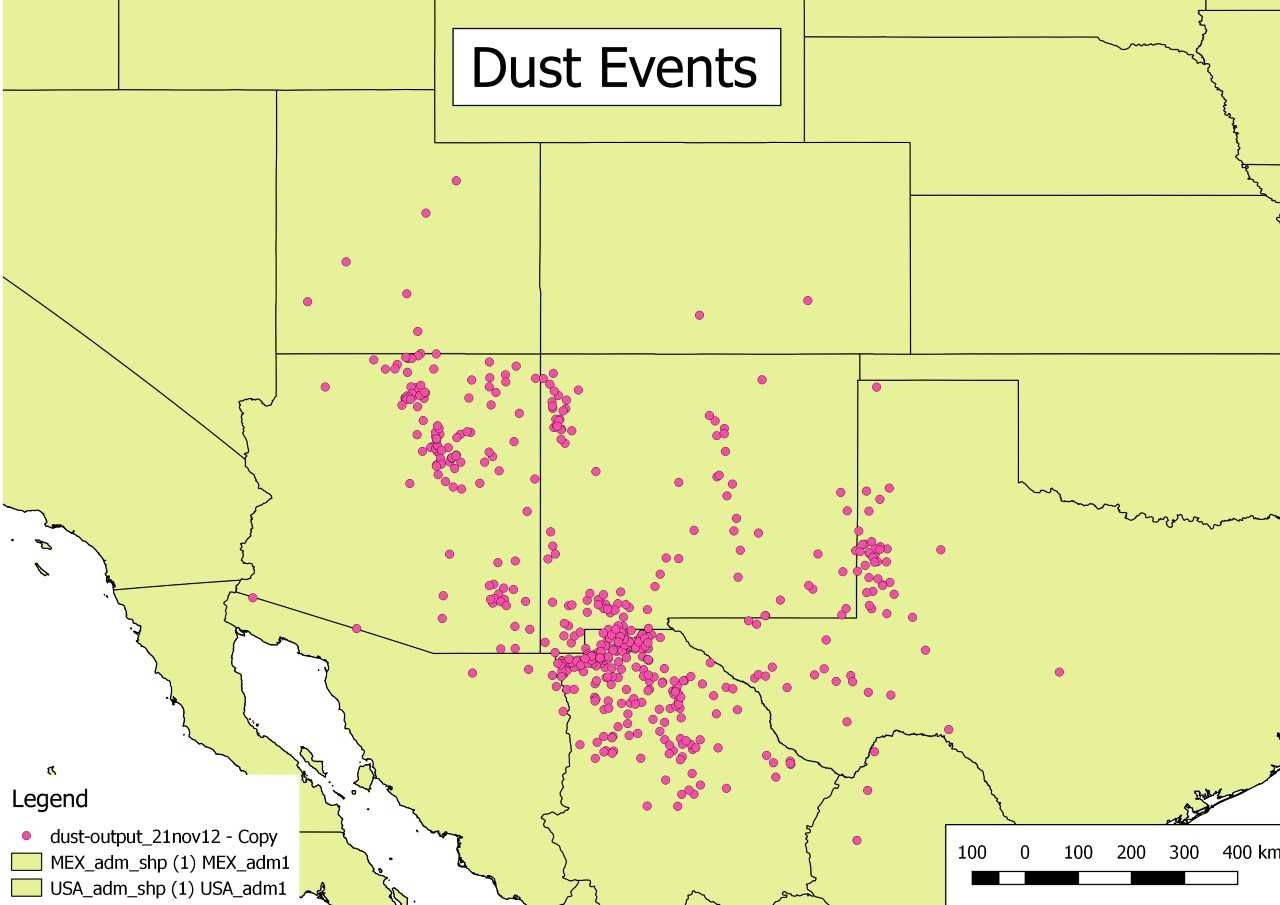
\includegraphics[width=\textwidth]{images/dustevents.jpg}
	\end{columns}
\end{frame}

\begin{frame}
	\frametitle{GRIB Example}
	\centering
	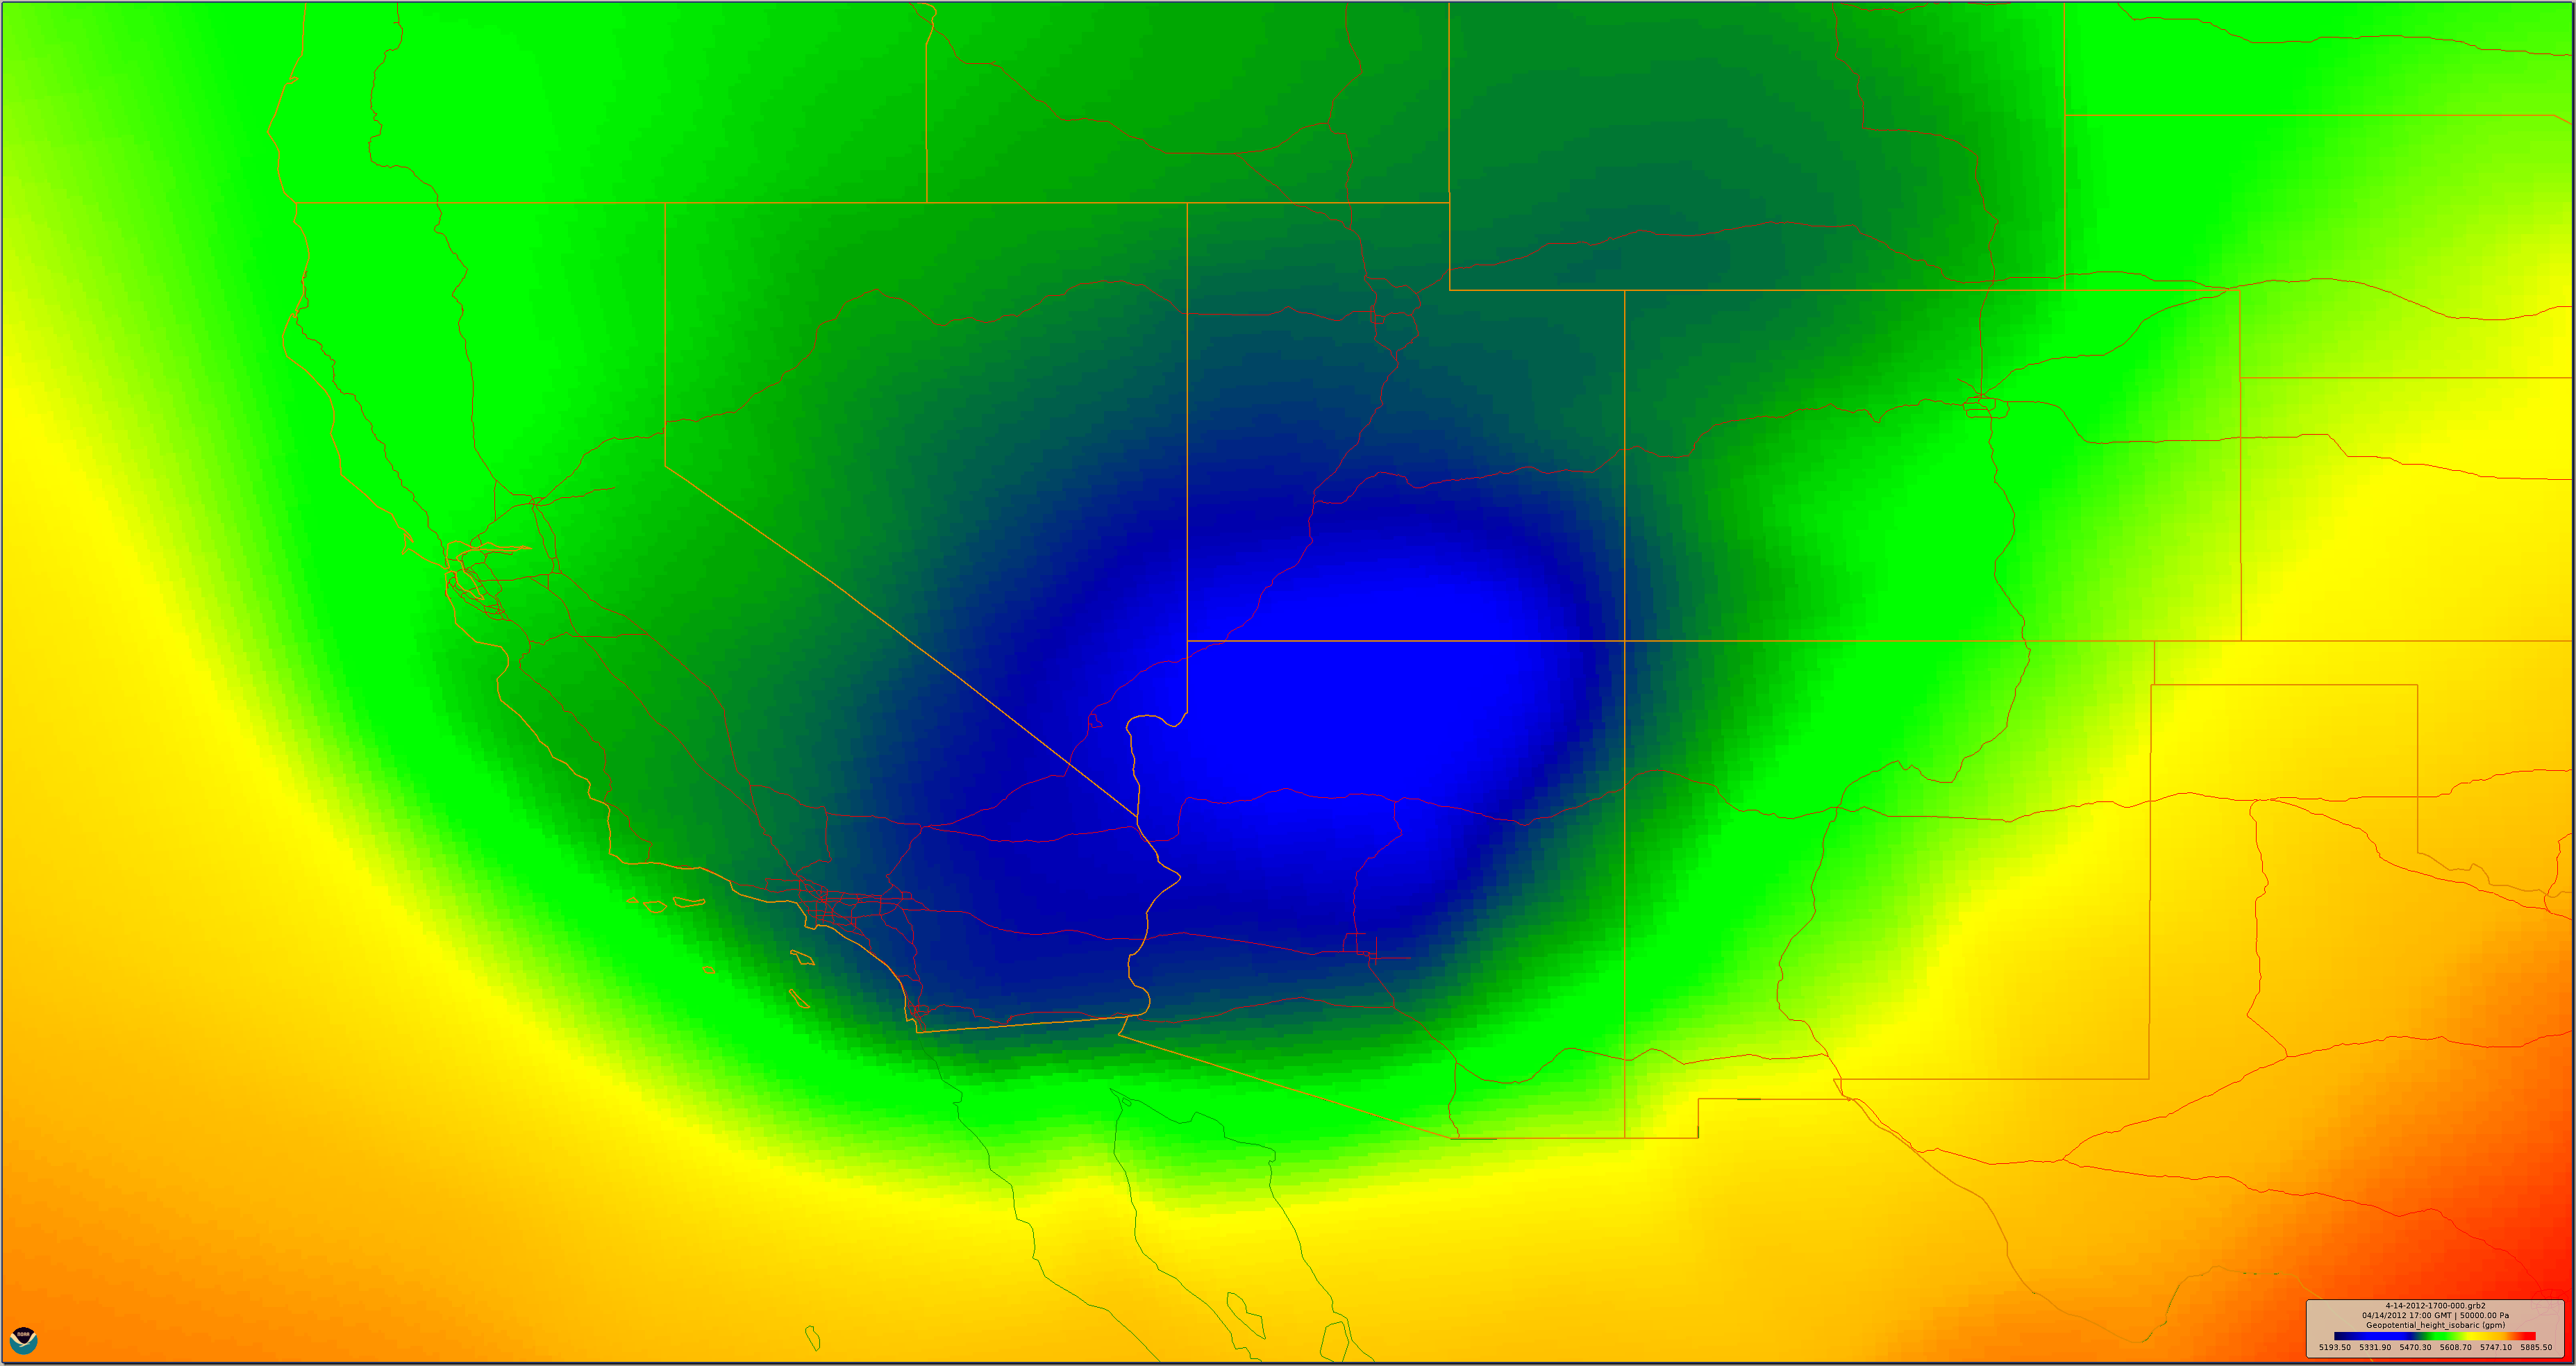
\includegraphics[width=0.75\textwidth]{images/abqlow.png}

	A single parameter's raster shown using NOAA Weather and Climate Tool. This image shows the 500mB geopotential height at 18:00GMT preceding a dust event on April 14, 2012 [4].


\end{frame}
\begin{frame}
	\frametitle{Reading GRIB files}
	\begin{itemize}
		\item
			pygrib Python library -- allows opening of .grb, .grb2 files in Python
		\item
			Opening a GRIB creates a file iterator, with each object in it a weather parameter [5].
		\item
			Each weather parameter has various attributes, including a raster of latitudes/longitudes and data for the parameter.
		\item
			Weather data gets stored into CSV files for easier lookup.
	\end{itemize}

\end{frame}
\begin{frame}
	\frametitle{PCA}
	\begin{itemize}
		\item
			Principal component analysis reduces the dimensionality of the data.
		\item 
			Transforms data into subspaces with the most spread between points - explains most of the variance in the data.
		\item
			RUC dataset has 315 dimensions for each instance -- could make algorithms less effective (curse of dimensionality).
		\item
			Normalize principal components for use in NN.


	\end{itemize}

\end{frame}

\begin{frame}
	\frametitle{PCA plots}
	\begin{columns}
		\column{0.5\textwidth}
		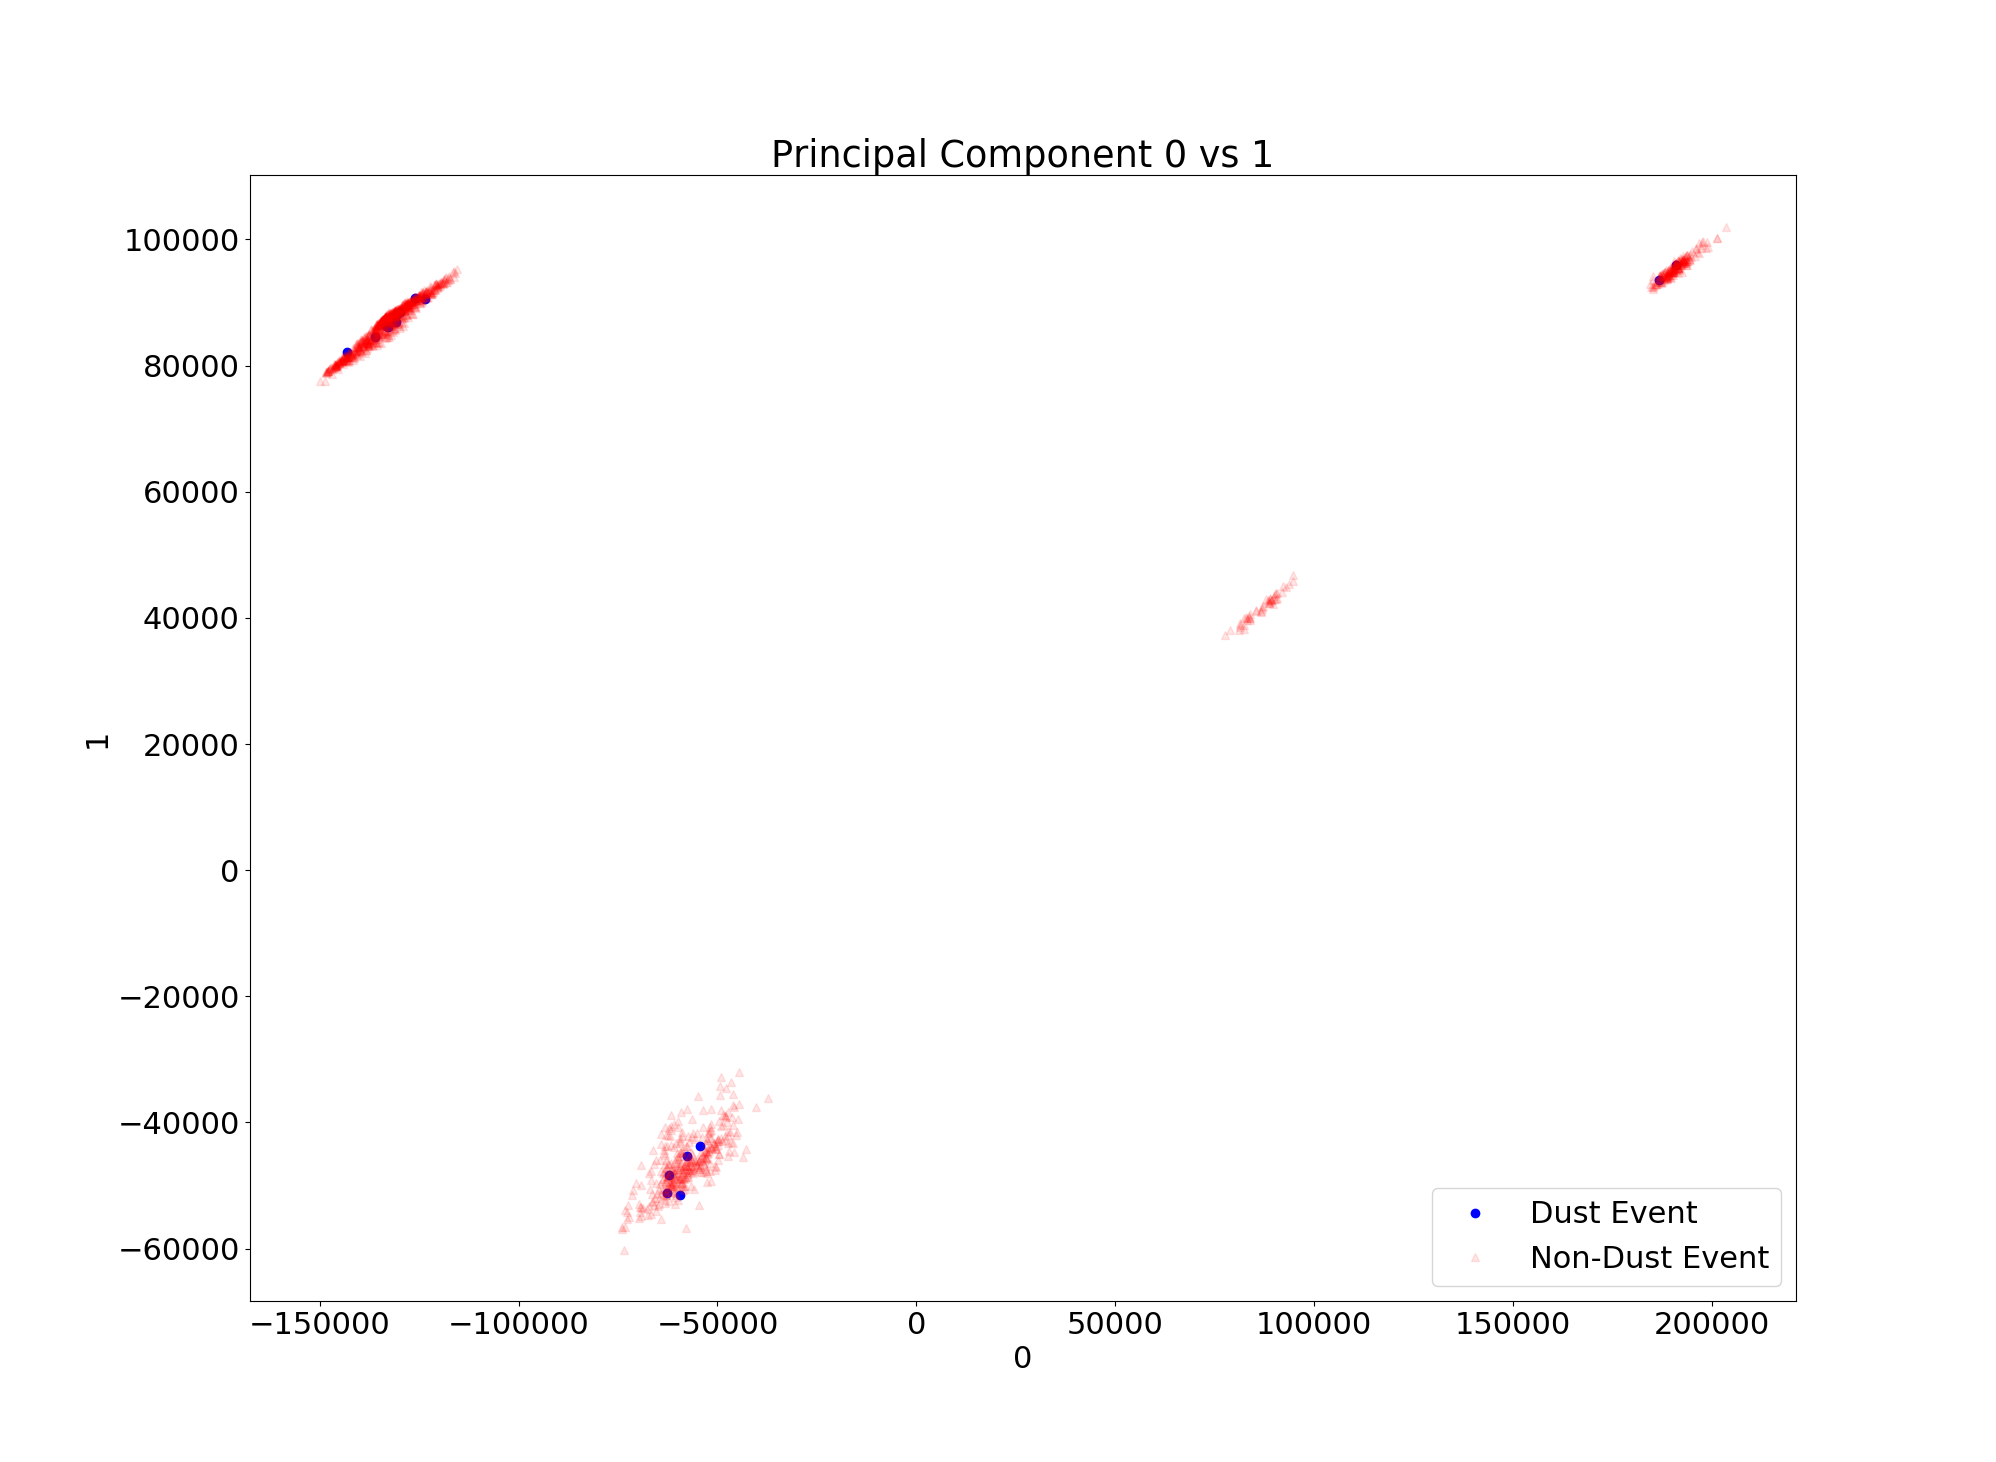
\includegraphics[width=\textwidth]{images/0vs1.png}
		\column{0.5\textwidth}
		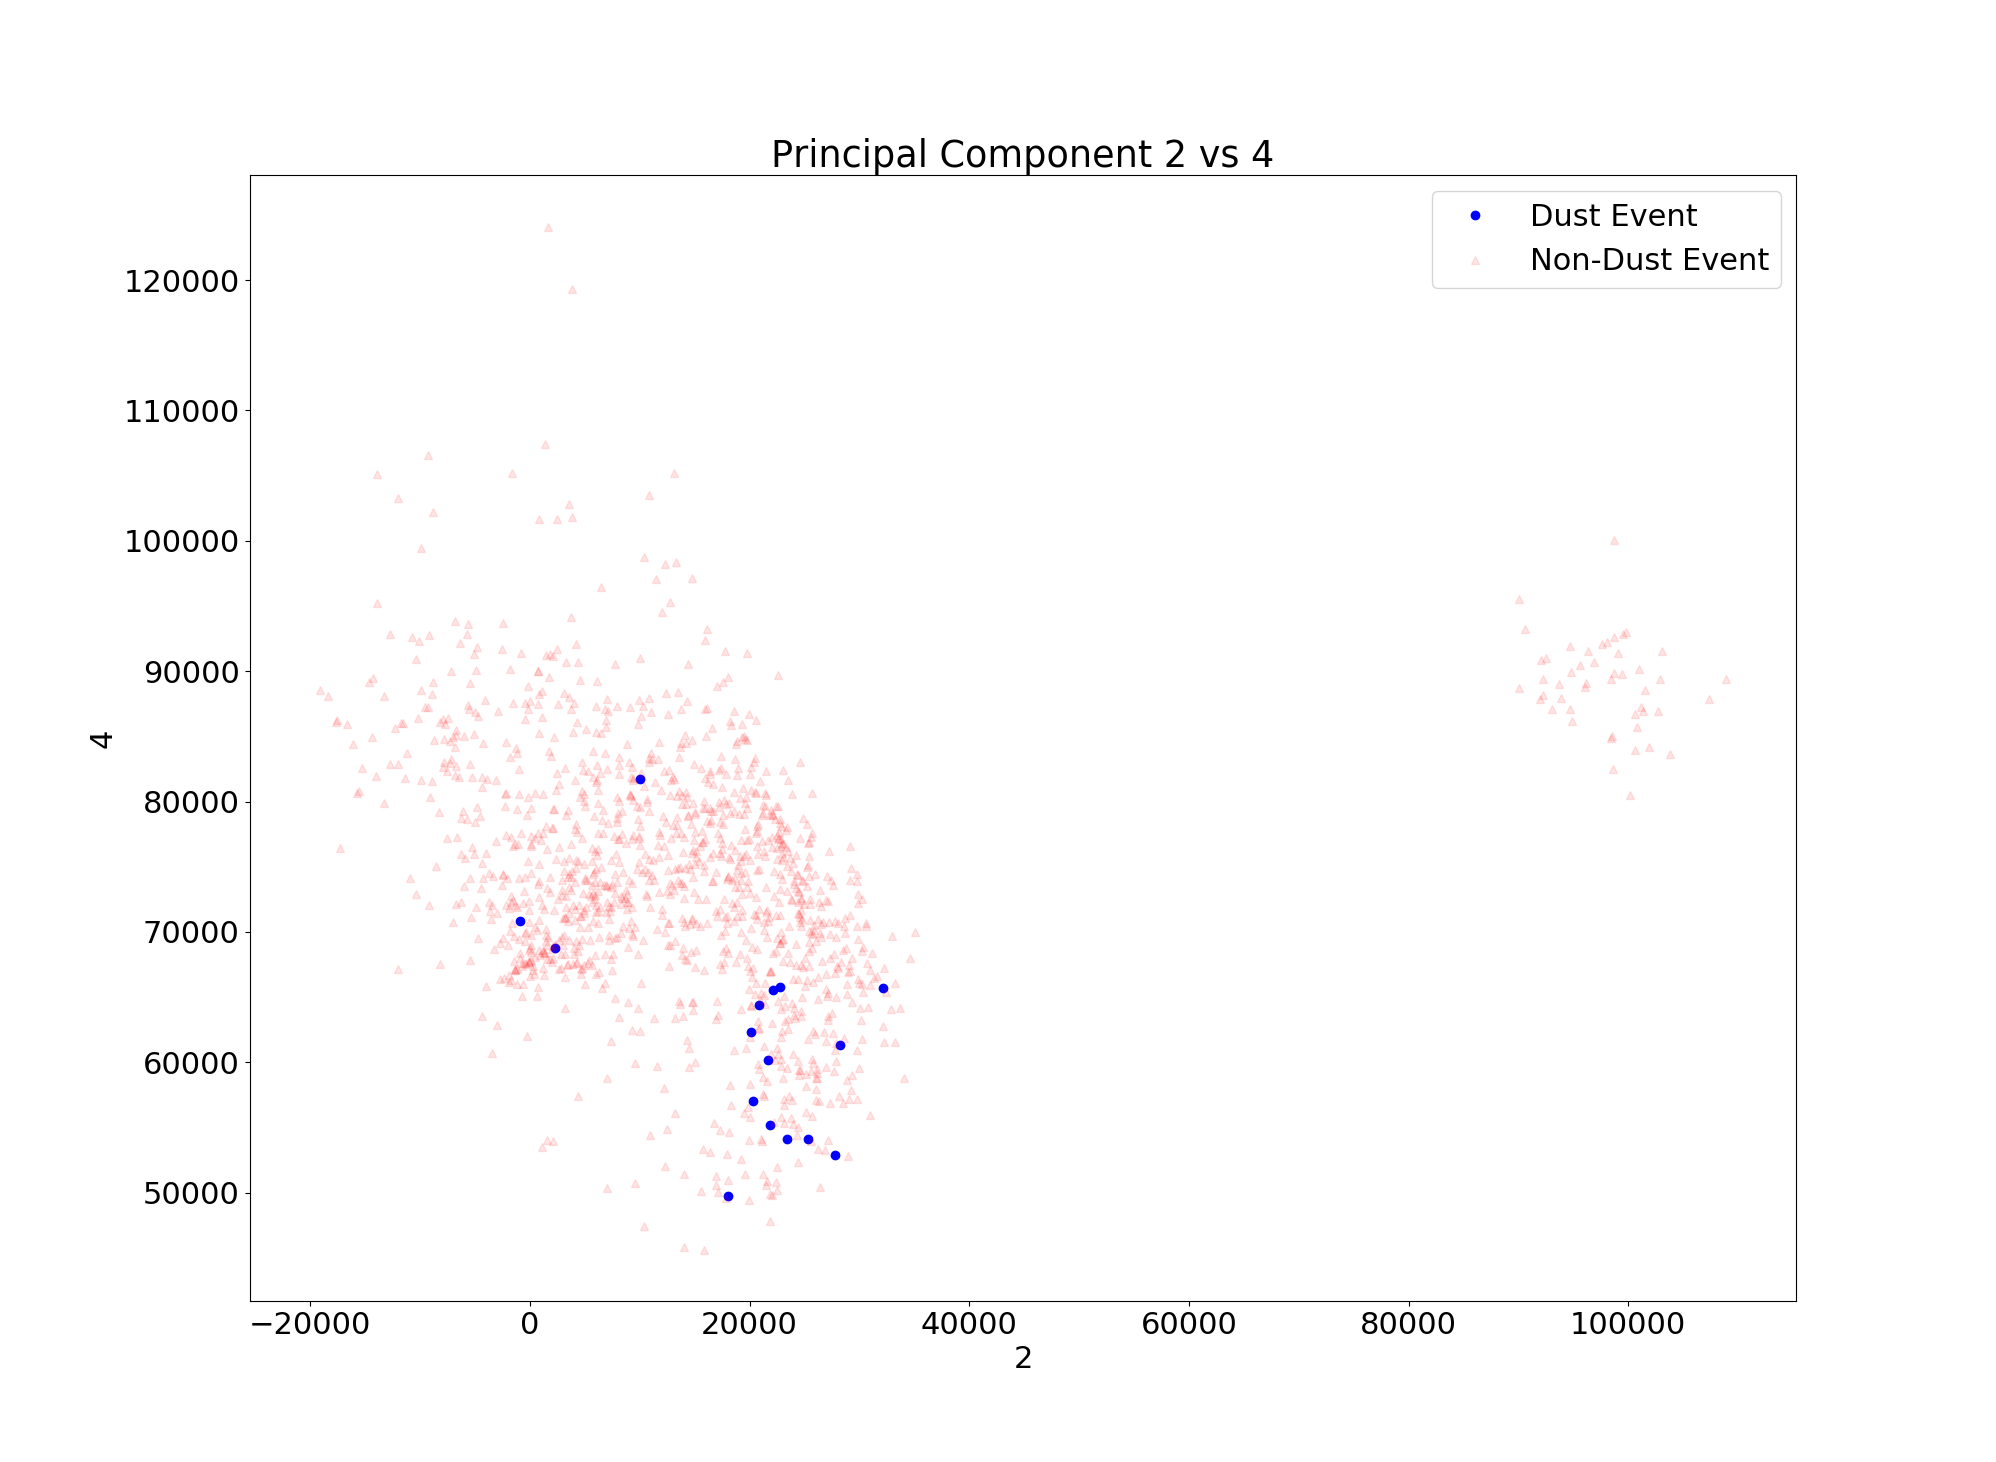
\includegraphics[width=\textwidth]{images/2vs4.png}
	\end{columns}

	Plots of principal components against each other. Left shows little no distinction between dust and non-dust events, while right shows some.
\end{frame}

\begin{frame}
	\frametitle{Algorithms}
	\begin{columns}
		\column{0.5\textwidth}
		\begin{itemize}
			\item
				Feedforward NN with PCA
			\item
				RNN/LSTM with PCA
		\end{itemize}

		Try each algorithm and see which one provides the best accuracy.
		\column{0.5\textwidth}
		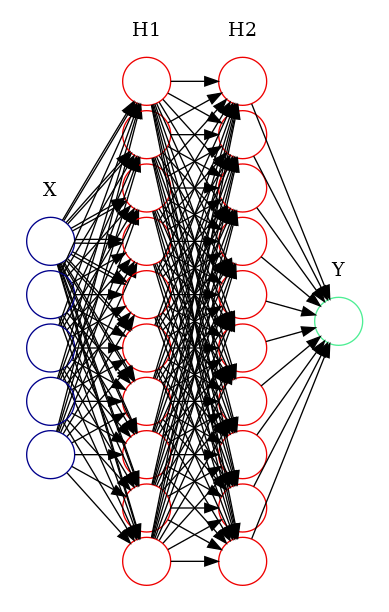
\includegraphics[width=0.75\textwidth]{images/nngraph.png}
	\end{columns}
\end{frame}
\begin{frame}
	\frametitle{Implementation of algorithms}
	\begin{columns}
		\column{0.5\textwidth}
		\begin{itemize}
			\item
				TensorFlow Python library
			\item
				Machine learning utility for creating computation graphs, doing lazy evaluations, using GPU for faster processing.
			\item
				Automates backpropagation and optimization algorithms [6].
		\end{itemize}
		\column{0.5\textwidth}
		
\includegraphics[width=\textwidth]{images/tensorflow.png}
	\end{columns}
\end{frame}
\begin{frame}
	\frametitle{Feedforward Neural Network}
	\begin{columns}
		\column{0.5\textwidth}
		\begin{itemize}
			\item
				10 principal components as inputs
			\item
				25 nodes per hidden layer
			\item
				2 output nodes
			\item
				Tested between 1 and 8 hidden layers
				
		\end{itemize}
		\column{0.5\textwidth}
		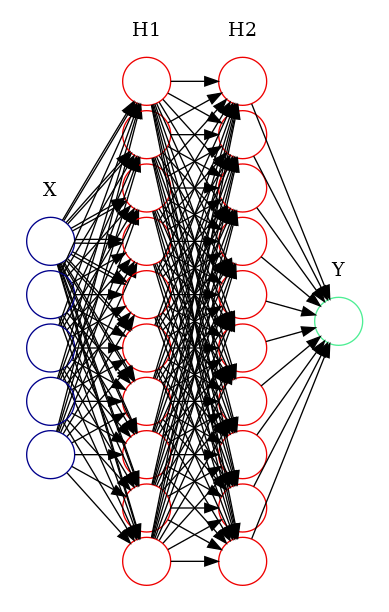
\includegraphics[width=0.75\textwidth]{images/nngraph.png}
	\end{columns}
\end{frame}
\begin{frame}
	\frametitle{Feedforward Neural Network, cont'd}
	\begin{columns}
		\column{0.5\textwidth}
		\begin{itemize}
			\item
				Use tanh activation function for hidden layers - steeper optimization gradient [7]
			\item
				Sigmoid output layer for values between 0 and 1
			\item
				Makes classification based on greatest value in output layer
			\item
				Weighted cross-entropy with logits loss function - weigh output losses according to imbalance in data set - about 11\% of events are dust.
		\end{itemize}
		\column{0.5\textwidth}
		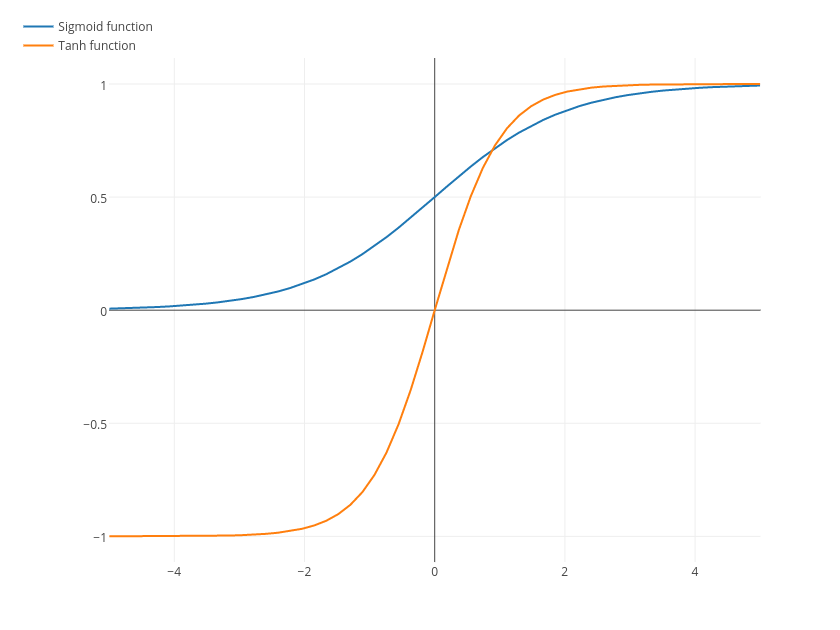
\includegraphics[width=\textwidth]{images/sigmoid-function-vs-tanh-function.png}
	\end{columns}
\end{frame}
\begin{frame}
	\frametitle{LSTM}
	Long short-term memory (LSTM) - RNN that stores past predictions in memory to create a more context-sensitive prediction. [8]
	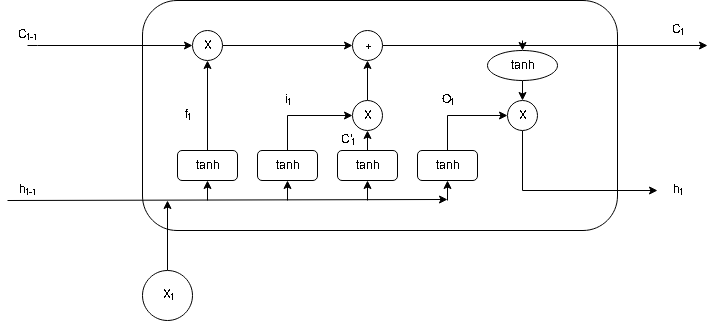
\includegraphics[width=\textwidth]{images/LSTMCell.png}
\end{frame}
\begin{frame}
	\frametitle{Feedforward Results, 1}
	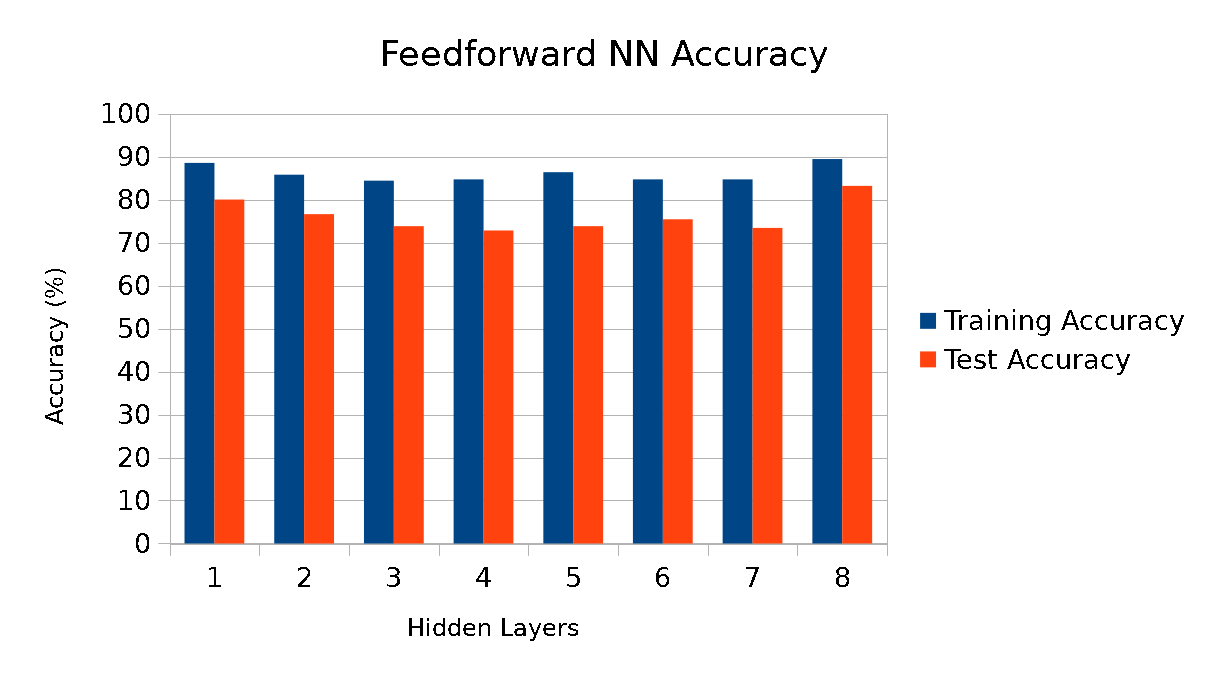
\includegraphics[width=\textwidth]{images/ffacc.png}
\end{frame}
\begin{frame}
	\frametitle{Feedforward Results, 2}
	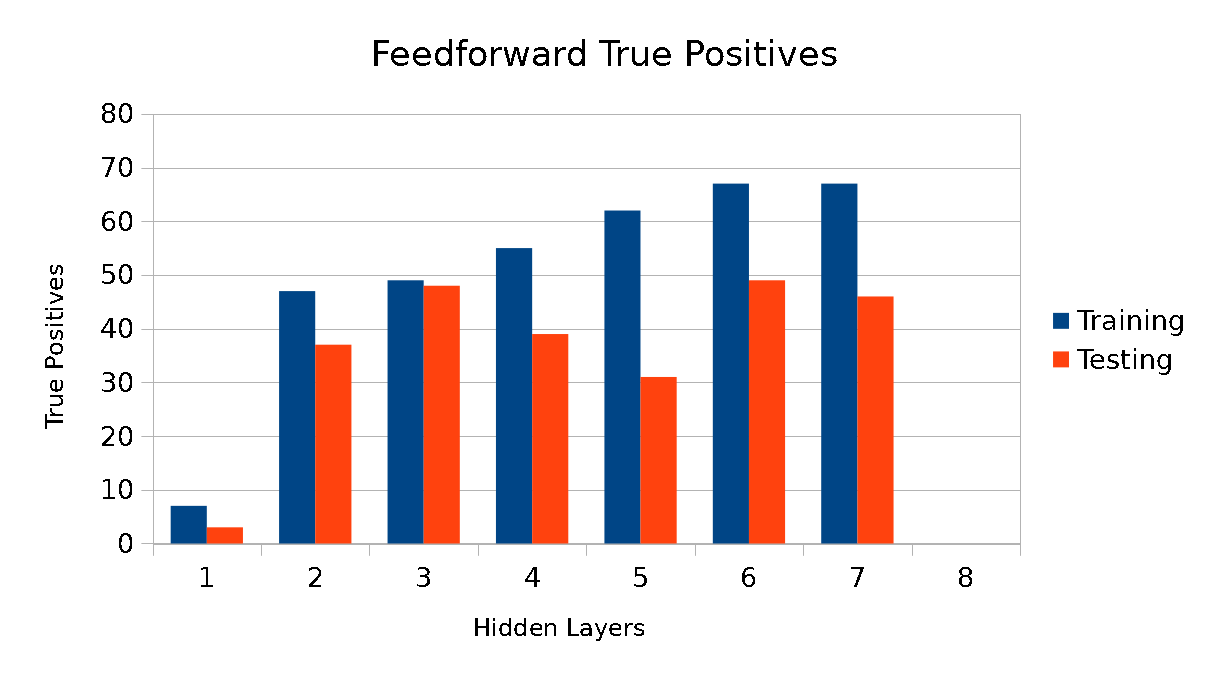
\includegraphics[width=\textwidth]{images/truepos.png}
\end{frame}
\begin{frame}
	\frametitle{Feedforward Results, 3}
	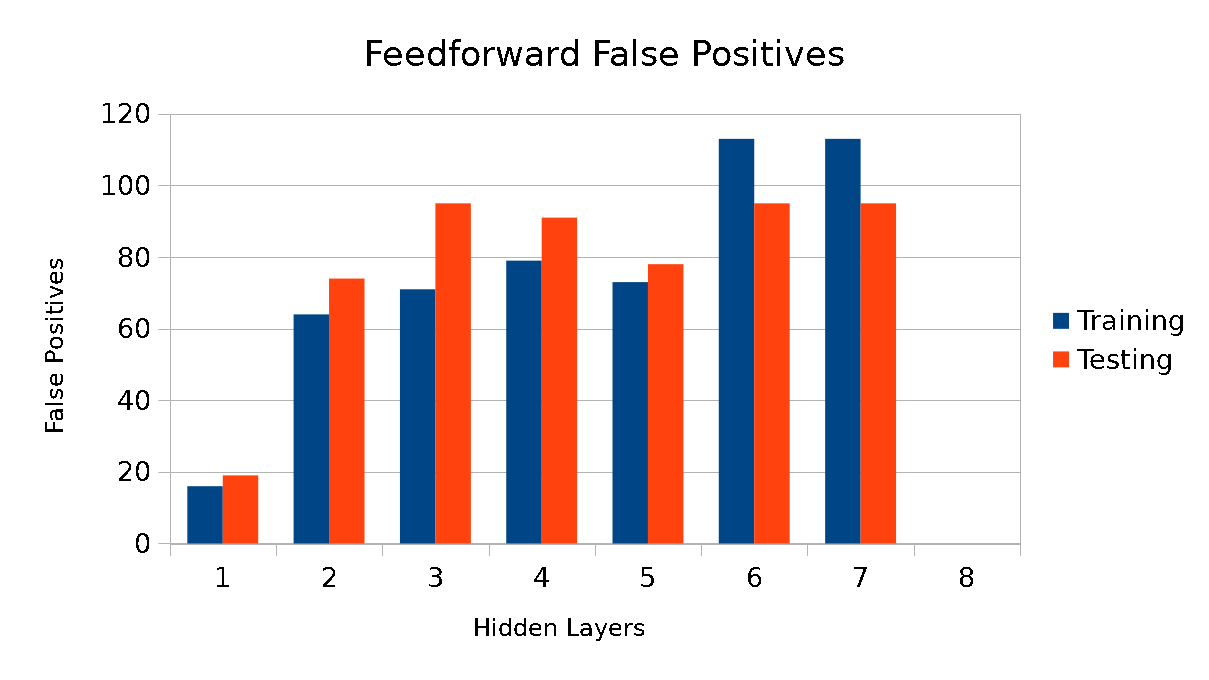
\includegraphics[width=\textwidth]{images/falsepos.png}
\end{frame}
\begin{frame}
	\frametitle{LSTM Results}
	\begin{itemize}
		\item 89.4685\% training accuracy - but one problem:
		\item Guessed negative on every prediction!
		\item Could be possible that even with compensation in loss function, the imbalanced data set makes it easier for the RNN to assume that every event is non-dust.
	\end{itemize}
\end{frame}
\begin{frame}
	\frametitle{Conclusion}
	\begin{itemize}
		\item
			Feedforward provides good preliminary results - 80-85\% training accuracy; potential for more accurate models.
		\item
			Current version of LSTM did not work as hoped - future models with a 1-hour resolution that predict 24-hour sequences may work better.
		\item
			Possibility for predictions off of raster images using RNN or CNN models.
	\end{itemize}
\end{frame}

\begin{frame}
	\frametitle{References}
	\small
	[1] UNEP GEAS. "Forecasting and early warning of dust storms." UNEP. Feb. 2013. Web. May 24 2017.

	[2] Armenta, Rebecca B. "Geopotential height patterns at 500mb associated with dust storms in the United States/Mexico border region during January-May of 2011-2014." May 2016 New Mexico State University.  Access May 31 2017.

	[3] "GNU Wget 1.18 Manual." GNU Project. Web. Jun. 27 2017.

	[4] "Rapid Refresh (RAP)." National Centers for Envrionmental Information. NOAA. Web. Jun. 27. 2017.

	[5] "pygrib documentation." Github. Dec. 29 2014. Web. Jun. 14 2017.

	[6] "Getting Started with TensorFlow." TensorFlow. Web. Jul. 5 2017.
	
	[7] LeCun, Y. et. al. "Efficient BackProp." Yann LeCun's Home Page. Web. Jul. 25 2017.

	[8] Olah, C. "Understanding LSTM Networks." Colah's blog. Aug. 27 2015. Web. Jul. 20 2017.

\end{frame}
\end{document}
